\documentclass{beamer}
\usetheme[
  numbering=fraction,
  background=light
]{metropolis} % Use metropolis theme

% Slide white area = 128 mm x 85.58 mm

\usepackage{tikz}
\usetikzlibrary{positioning}
\usepackage{booktabs}
\usepackage{multirow}
\usepackage{fontawesome}

\newcommand{\slideheight}{85.58mm}
\newcommand{\slidewidth}{128mm}
\newcommand{\southsep}{1.4mm}

\title{Design of the frontend for LEN5,\\a RISC-V Out-of-Order processor}

\makeatletter
\setbeamertemplate{title page}{
  \begin{minipage}[b][\paperheight]{\textwidth}
    \vfill%
    \ifx\inserttitle\@empty\else\usebeamertemplate*{title}\fi
    \ifx\insertsubtitle\@empty\else\usebeamertemplate*{subtitle}\fi
    \usebeamertemplate*{title separator}
    \ifx\beamer@shortauthor\@empty\else\usebeamertemplate*{author}\fi
    %\ifx\insertdate\@empty\else\usebeamertemplate*{date}\fi
    \ifx\insertinstitute\@empty\else\usebeamertemplate*{institute}\fi
    \vfill
    \vspace*{6cm}
  \end{minipage}
}
\makeatother

\begin{document}
\begin{frame}[plain]
  \maketitle
  \begin{tikzpicture}[overlay, remember picture]
    \node[below=0cm of current page.center]
      {\includegraphics[width=4.5cm]{img/out.png}};
    \node[above right=0.5cm and 1cm of current page.west,align=left]
      {Candidate:\\Marco Andorno};
    \node[above left=0.5cm and 1cm of current page.east,align=right]
      {Supervisor:\\prof. Maurizio Martina};
    \node[below=2.5cm of current page.center,align=center]
      {\small Master's thesis in Electronic Engineering\\\small Academic year 2018-2019};
  \end{tikzpicture}
\end{frame}
\addtocounter{framenumber}{-1}

\section{LEN5 overview}

\begin{frame}{First Frame}
  Hello, world!
\end{frame}

\section{Frontend design}

\begin{frame}{Frontend overview}
  \begin{tikzpicture}[overlay, remember picture]
    \node[below=\southsep of current page.south,anchor=south] {
      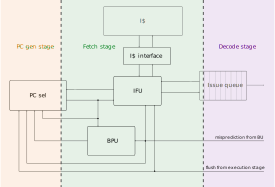
\includegraphics[width=\slidewidth,
                        height=\slideheight]{img/frontend.pdf}
    };
  \end{tikzpicture}
\end{frame}

\begin{frame}{PC gen stage}
  \begin{tikzpicture}[overlay, remember picture]
    \node[below=\southsep of current page.south,anchor=south] {
      \includegraphics[keepaspectratio,
                        width=\slidewidth,
                        height=\slideheight]{img/pc_gen_stage.pdf}
    };
  \end{tikzpicture}
\end{frame}

\begin{frame}{Instruction Fetch Unit (IFU)}
  \begin{tikzpicture}[overlay, remember picture]
    \node[below=\southsep of current page.south,anchor=south] {
      \includegraphics[keepaspectratio,
                        width=\slidewidth,
                        height=\slideheight]{img/ifu.pdf}
    };
  \end{tikzpicture}
\end{frame}

\section{Branch management}

\begin{frame}{Branch Prediction Unit (BPU)}
  \begin{tikzpicture}[overlay, remember picture]
    \node[below=\southsep of current page.south,anchor=south] {
      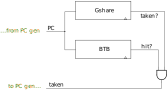
\includegraphics[keepaspectratio,
                        width=\slidewidth,
                        height=\slideheight]{img/bpu-idea.pdf}
    };
  \end{tikzpicture}
\end{frame}

\begin{frame}{Gshare branch predictor}
  \begin{tikzpicture}[overlay, remember picture]
    \node[below=\southsep of current page.south,anchor=south] {
      \includegraphics[keepaspectratio,
                        width=\slidewidth,
                        height=\slideheight]{img/gshare.pdf}
    };
  \end{tikzpicture}
\end{frame}

\begin{frame}{Branch Target Buffer (BTB)}
  \begin{tikzpicture}[overlay, remember picture]
    \node[below=\southsep of current page.south,anchor=south] {
      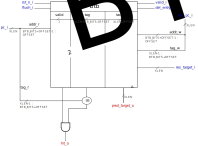
\includegraphics[keepaspectratio,
                        width=\slidewidth,
                        height=\slideheight]{img/btb.pdf}
    };
  \end{tikzpicture}
\end{frame}

\begin{frame}{Branch unit}
  \begin{tikzpicture}[overlay, remember picture]
    \node[below=\southsep of current page.south,anchor=south] {
      \includegraphics[keepaspectratio,
                        width=\slidewidth,
                        height=\slideheight]{img/branch_unit.pdf}
    };
  \end{tikzpicture}
\end{frame}

\begin{frame}{BPU update actions}
  \begin{table}
    \makebox[\textwidth][c]{
      \begin{tabular}{llll}
        \toprule
        \textbf{Prediction}         & \textbf{Resolution}         & \textbf{Target}             & \textbf{Action} \\
        \midrule
        \multirow{7}{*}{Taken}      & \multirow{4}{*}{Taken}      & \faCheck                    & Increment 2-bit counter \\
        \cline{3-4}
                                    &                             & \multirow{3}{*}{\faRemove}  & Increment 2-bit counter \\
                                    &                             &                             & Update BTB entry \\
                                    &                             &                             & Flush, go to right target \\
        \cline{2-4}
                                    & \multirow{3}{*}{Not taken}  & \multirow{3}{*}{\faMinus}   & Decrement 2-bit counter \\
                                    &                             &                             & Remove BTB entry \\
                                    &                             &                             & Flush, go to branch PC+4 \\
        \midrule
        \multirow{4}{*}{Not taken}  & Not taken                   & \faMinus                    & Decrement 2-bit counter \\
        \cline{2-4}
                                    & \multirow{3}{*}{Taken}      & \multirow{3}{*}{\faMinus}   & Increment 2-bit counter \\
                                    &                             &                             & Add BTB entry \\
                                    &                             &                             & Flush, go to right target \\
        \bottomrule          
      \end{tabular}
      }
  \end{table}
\end{frame}

\section{Results}

\end{document}